\chapter{Evaluation}
\label{cha:evaluation}
%Eine Evaluation bzgl. Kommunikationsreichweiten, Anzahl „Agenten“ im Gebäude, oder Zeit bis zu vollständiger Evakuierung, etc. soll durchgeführt werden. Insbesondere sollte in der Evaluie-rung auf die Qualität der Lokalisierung in Abhängigkeit der Anzahl Notausgänge / Anchor Nodes, Anzahl Sensorknoten und der Kommunikationsreichweite eingegangen werden. 

\section{Lokalisierung}

Um die beste Lokalisierung mit dem Algorithmus zu erreichen, spielen die Parameter die größte Rolle. In den folgenden Tabellen und Analysen wird deutlich, wie groß die Unterschiede zwischen den verschiedenen Ausführungen sein kann, wenn man einen Parameter verändert. Zwischen den Lokalisierungen in einer Tabelle werden die Personen nicht neu generiert, die Werte in einer Tabelle sind also vergleichbar. Zwischen verschiedenen Tabellen werden die Personen jedoch neu generiert, also kann es zu generellen Abweichungen kommen, da die Verteilung der Personen auch eine Rolle in der Genauigkeit spielt.

\paragraph{Beschreibung der Parameter und Tabellenspalten}

\begin{description}
   \item[number-of-exits] (Tabellenspalte \emph{\#Exits}) \hfill \\
	Anzahl der Ausgänge und Sensorpunkte für den Algorithmus. Der Algorithmus soll mit mehr Sensorpunkten besser approxmieren, ab 3 ist eine realistische Berechnung überhaupt erst möglich.
   \item[personCount] (Tabellenspalte \emph{\#Person}) \hfill \\
	Anzahl der Personen in der Simulation. Eine Mindestanzahl ist nötig, um das Kommunikationsnetz aufzubauen. Mehr Personen bedeutet eine genauere Abschätzung der Distanzen zu den Sensorpunkten, da der Hop Counts zuverlässiger ist. Das ist durch die Verteilung der Personen gegeben, bei sehr vielen Personen ist die Chance höher, das die Hop Counts \emph{normaler} verteilt sind.
   \item[detection-radius] (Tabellenspalte \emph{detRad}) \hfill \\
	Radius mit dem der UDG bestimmt wird. Das Attribut ist auch für den Hop Count verantwortlich, wenn man ihn höher wählt, dann ist der Hop Count für weiterstehende Personen kleiner, da der Kommunikationsradius höher ist. Ein kleinerer Wert könnte dazu führen, dass das Netz nicht vollständig alle Notausgänge und Personen verbindet, zu groß führt zu einem ungenauen Hop Count.
   \item[locate-iterations] (Tabellenspalte \emph{\#iter}) \hfill \\
	Wieviele Iterationen der Algorithmus durchläuft. Mehr Iterationen bedeutet höhere Genauigkeit, aber auch höherer Rechenaufwand.
   \item[approx-dist] (Tabellenspalte \emph{~dist}) \hfill \\
	Die Distanz die der Algorithmus zu jedem Hop Count annimmt. Die Zahl ist abhängig von der Personendichte und dem detection-radius.
   \item[average-estimated-distance] (Tabellenspalte \emph{avgDist}) \hfill \\
	Durchschnittlicher Abstand aller geschätzten Positionen zu der tatsächlichen Position. 
   \item[min-estimated-distance] (Tabellenspalte \emph{minDist}) \hfill \\
	Kleinste Distanz von einer geschätzten Position zu einer genauen Position, d.h. die am besten geschätzte Position.
   \item[max-estimated-distance] (Tabellenspalte \emph{maxDist}) \hfill \\
	Größte Distanz von einer geschätzten Position zu einer genauen Position, d.h. die am schlechtesten geschätzte Position.
\end{description}

\begin{table}[h]
\begin{tabular}{|l|l|l|l|l|l|l|l|l|}
\hline
No & \#Exits & \#Person & detRad & \#iter & ~dist & avgDist & minDist & maxDist \\ \hline
1  & 3       & 100      & 50     & 5      & 15    & 52,13   & 10,22   & 126,51  \\ \hline
2  & 3       & 100      & 50     & 5      & 30    & 35,23   & 3,33    & 115,85  \\ \hline
3  & 3       & 100      & 50     & 5      & 35    & 38,65   & 3,24    & 121,78  \\ \hline
4  & 3       & 100      & 50     & 10     & 15    & 52,87   & 10,56   & 126,47  \\ \hline
5  & 3       & 100      & 50     & 10     & 30    & 34,44   & 4,69    & 105,88  \\ \hline
6  & 3       & 100      & 50     & 10     & 35    & 28,18   & 1,84    & 109,89  \\ \hline
7  & 3       & 100      & 50     & 20     & 15    & 52,49   & 10,96   & 126,95  \\ \hline
8  & 3       & 100      & 50     & 20     & 30    & 33,75   & 4,44    & 90,54   \\ \hline
9  & 3       & 100      & 50     & 20     & 35    & 22,95   & 1,81    & 82,22   \\ \hline
10 & 3       & 100      & 50     & 30     & 15    & 52,82   & 10,91   & 126,36  \\ \hline
11 & 3       & 100      & 50     & 30     & 30    & 33,21   & 4,45    & 80,27   \\ \hline
12 & 3       & 100      & 50     & 30     & 35    & 20,1    & 1,17    & 66,19   \\ \hline
\end{tabular}
\caption{Evaluierung für raumplan.png mit 3 Exits und 100 Personen}
\label{fig:eva01}
\end{table}

An der Tabelle \ref{fig:eva01} kann man bei den Anzahl der Iterationen sehen, wie die Genauigkeit des Algorithmus mit der Anzahl der Iterationen steigt. Zwischen 5 und 20 Iterationen ist eine Verbesserung von 50\% zu sehen, wenn die approx-dist dementsprechend gewählt wurde. Von 20 auf 30 Iterationen ist die Verbesserung in Relation mit dem Rechenaufwand wohl irrelevant. In den zukünfiigen Experimenten sei die Anzahl der Iterationen stets 20.


\begin{table}[h]
\begin{tabular}{|l|l|l|l|l|l|l|l|l|}
\hline
No & \#Exits & \#Person & detRad & \#iter & ~dist & avgDist & minDist & maxDist \\ \hline
13 & 3       & 150      & 30     & 20     & 15    & 41,15   & 2,57    & 88,11   \\ \hline
14 & 3       & 150      & 30     & 20     & 17    & 35,55   & 4,45    & 72,51   \\ \hline
15 & 3       & 150      & 30     & 20     & 19    & 27,51   & 4,23    & 52,65   \\ \hline
16 & 3       & 150      & 30     & 20     & 20    & 23,46   & 2,37    & 58,46   \\ \hline
\end{tabular}
\caption{Evaluierung für raumplan.png mit 3 Exits und 150 Personen}
\label{fig:eva02}
\end{table}

An der Tabelle \ref{fig:eva02} wird der Effekt von verschiedenen approx-dist Werten veranschaulicht. Man findet eine gute Approximation bei \( \frac{2}{3} \) vom Detection Radius. Wenn ie approx-dist noch höher gewählt wird, fallen zuviele geschätzte Position außerhalb der Simulationsumgebung an und das Ergebnis wird verfälscht. Dabei muss noch beachtet werden, dass der detection-radius gesenkt werden konnte, da nun mehr Personen vorhanden sind, die im Kommunikationsnetz den Hop Count genauer weiterreichen und repräsentieren können.


\begin{table}[h]
\begin{tabular}{|l|l|l|l|l|l|l|l|l|}
\hline
No & \#Exits & \#Person & detRad & \#iter & ~dist & avgDist & minDist & maxDist \\ \hline
17 & 3       & 200      & 25     & 20     & 15    & 21,56   & 1,25    & 62,25   \\ \hline
18 & 3       & 200      & 25     & 20     & 17    & 14,59   & 1,64    & 36,32   \\ \hline
19 & 3       & 200      & 25     & 20     & 19    & 22,14   & 2,31    & 66,81   \\ \hline
\end{tabular}
\caption{Evaluierung für raumplan.png mit 3 Exits und 200 Personen}
\label{fig:eva03}
\end{table}

Bei der Tabelle \ref{fig:eva03} ist verdeutlicht, dass bei einer größeren Anzahl von Personen eine höhere Dichte entsteht und durch einen kleineren detection-radius zusammen mit einem passenden approx-dist wesentlich genauere Positionen gefunden werden können. Hier ist auch erneut zu sehen, dass \( \frac{2}{3} \) vom Detection Radius wohl ein sinnvoller Wert ist, gegeben einem sinnvollen detection-radius, der nicht viel zu hoch ist, für die vorliegende Dichte der Personen. In den folgenden Experimenten bleiben wir bei 200 Personen mit einem detection-radius von 25.

\begin{table}[h]
\begin{tabular}{|l|l|l|l|l|l|l|l|l|}
\hline
No & \#Exits & \#Person & detRad & \#iter & ~dist & avgDist & minDist & maxDist \\ \hline
20 & 6       & 200      & 25     & 20     & 15    & 21,72   & 0,65    & 48,62   \\ \hline
21 & 6       & 200      & 25     & 20     & 17    & 12,78   & 1,14    & 35,02   \\ \hline
22 & 6       & 200      & 25     & 20     & 19    & 10,17   & 0,76    & 57,57   \\ \hline
\end{tabular}
\caption{Evaluierung für raumplan.png mit 6 Exits und 200 Personen}
\label{fig:eva04}
\end{table}

In Tabelle \ref{fig:eva04} wird deutlich, wie wichtig es ist viele gleichverteilte Orientierungspunkte zu haben für den Algorithmus. Die Genauigkeit ist deutlich höher im Mittel, insbesondere der kleinste und größte Abstand ist wesentlich besser.

\begin{table}[h]
\begin{tabular}{l|l|l|l|l|l|l|l|l|}
\cline{2-9}
No & \#Exits & \#Person & detRad & \#iter & ~dist & avgDist & minDist & maxDist \\ \cline{2-9} 
23 & 9       & 200      & 25     & 20     & 15    & 18,35   & 1,64    & 42,25   \\ \cline{2-9} 
24 & 9       & 200      & 25     & 20     & 17    & 11,08   & 0,78    & 28,35   \\ \cline{2-9} 
25 & 9       & 200      & 25     & 20     & 19    & 18,03   & 1,25    & 41,47   \\ \cline{2-9} 
\end{tabular}
\caption{Evaluierung für raumplan.png mit 9 Exits und 200 Personen}
\label{fig:eva05}
\end{table}

Bei Tabelle \ref{fig:eva05} mit 9 Exits ist noch eine Verbesserung zu sehen, inbesondere wieder in der min und max distance. Bei mehr Orientierungspunkten, einem dichteren Netzwerk und mehr Personen wäre eine Genauigkeit auf wenige Patches genau problemlos möglich.

\section{Evakuierungsdauer}
Um die Evakuierungsdauer zu evaluieren wird ein Szenario erstellt, bei dem sich 100 oder 200 Personen zusammen mit 20 Gasbomben auf der IKG-Etage befinden. Eine Gasausbreitung findet allerdings nicht statt. 

Wir schauen, wie schnell die Personen von der Etage flüchten können. Die Voraussetzungen sind, dass ein vollständiger UDG gegeben ist, das heißt bei 100 Personen wird ein detection-radius von 35 angenommen, bei 200 einer von 25, weil der in ausreichend Fällen einen vollständigen Graphen im Ausgangszustand erzeugt. Es wird mit 3, 6 und 9 Notausgängen geprüft. 

Es wird dabei überprüft, wie schnell die Personen sich mit Hilfe des Kommunikationsnetzes, den zellulären Automaten und der Notausgänge retten können. Die verschiedenen Personen und Notausgänge, sowie die verschiedenen Anordnungen der Personen stellen dabei den natürlichen Arbeitsablauf in einem Bürogebäude da und machen die Evaluierungsergebnisse interessant und relevant.

\begin{table}[h]
\begin{tabular}{c|c|c|c|c|c|c|c|c|c|c|c|c|}
\cline{2-13}
                           & \multicolumn{6}{|c}{100 Personen}                                                          & \multicolumn{6}{|c|}{200 Personen}                                                          \\ \cline{2-13} 
                           & \multicolumn{2}{|c}{3 Exits} & \multicolumn{2}{|c}{6 Exits} & \multicolumn{2}{|c}{9 Exits} & \multicolumn{2}{|c}{3 Exits} & \multicolumn{2}{|c}{6 Exits} & \multicolumn{2}{|c|}{9 Exits} \\ \hline
\multicolumn{1}{|c|}{\#1}  & 44           & 298           & 18           & 174           & 15           & 166           & 19           & 226           & 18           & 171           & 16            & 160           \\ \hline
\multicolumn{1}{|c|}{\#2}  & 40           & 217           & 16           & 146           & 20           & 140           & 20           & 209           & 13           & 130           & 13            & 142           \\ \hline
\multicolumn{1}{|c|}{\#3}  & 45           & 246           & 18           & 143           & 14           & 138           & 18           & 207           & 16           & 163           & 10            & 122           \\ \hline
\multicolumn{1}{|c|}{\#4}  & 56           & 232           & 15           & 152           & 13           & 144           & 20           & 213           & 15           & 128           & 14            & 169           \\ \hline
\multicolumn{1}{|c|}{\#5}  & 35           & 305           & 16           & 135           & 16           & 180           & 22           & 206           & 13           & 140           & 14            & 135           \\ \hline
\multicolumn{1}{|c|}{\#6}  & 41           & 301           & 18           & 145           & 18           & 126           & 17           & 203           & 14           & 150           & 17            & 120           \\ \hline
\multicolumn{1}{|c|}{\#7}  & 36           & 205           & 19           & 185           & 24           & 153           & 16           & 218           & 15           & 141           & 12            & 134           \\ \hline
\multicolumn{1}{|c|}{\#8}  & 39           & 190           & 15           & 165           & 12           & 137           & 16           & 191           & 14           & 130           & 13            & 147           \\ \hline
\multicolumn{1}{|c|}{\#9}  & 49           & 260           & 16           & 135           & 16           & 155           & 22           & 223           & 11           & 168           & 10            & 150           \\ \hline
\multicolumn{1}{|c|}{\#10} & 51           & 240           & 18           & 175           & 18           & 165           & 15           & 250           & 18           & 151           & 9             & 147           \\ \hline
\multicolumn{1}{|c|}{avg}  & 43,6         & 249,4         & 16,9         & 155,5         & 16,6         & 150,4         & 18,5         & 214,6         & 14,7         & 147,2         & 12,8          & 142,6         \\ \hline
\end{tabular}
\caption{Evaluierung der Evakuierungsdauer}
\label{fig:data}
\end{table}

Die Tabelle \ref{fig:data} zeigt die Ergebnisse der Simulation unter den gegeben Randbedingungen. Dabei ist die linke Spalte unter jeder Angabe der Anzahl der Exits die Ticks bis zur ersten geretteten Person, die rechte Spalte die Anzahl der vergangenen Ticks bis alle Personen gerettet wurden.

Besonders interessant an den Daten ist der Unterschied zwischen den Personen, obwohl die Anzahl der Personen verdoppelt wird, wird die Flucht aller Personen im Mittel schneller, da die Warnung im Netz schneller verbreitet wird. Das mehr Notausgänge bei einer Flucht helfen ist gegeben. Jedoch ist anzumerken, dass der Unterschied zwischen 6 und 9 Notausgänge nicht sehr hoch ist. Auch interessant ist bei wenigen Notausgängen und wenigen Personen die stärkeren Schwankungen zwischen Maximaldauer und Minimaldauer der Evakuierungen, die auf die Gegebenheit der zufälligen Bewegungen der Personen und des Kommunikationsnetzes zurückzuführen sind.

\section{Fazit}

Vor der Implementierung der Simulation stellten sich einige Fragen um das Thema: Kann mit einem Geosensornetz die Evakuierung eines Gebäudes beschleunigt werden? Welche Faktoren spielen eine Rolle? Was passiert, wenn Ereignisse über ein Netzwerk dezentral verschickt werden? Kann zuverlässig sichergestellt werden, das eine sichere Evakuierung trotzdem möglich ist? Ist es möglich anhand von Orientierungspunkten eine Position von Personen mit einem mobilen Gerät zuverlässig zu bestimmen? Diese Fragen wurden von der Simulation beantwortet; das Geosensornetz zeigt, dass selbst Personen die nicht unmittelbar in Gefahr schwebten durch das Netz gerettet werden konnten.

Leider stellten sich aber auch viele Probleme auf, man benötigt sehr viele Personen und Orientierungspunkte um eine sichere und zuverlässige Lokalisierung klar zustellten und selbst dann können Sammelplätze und Leerräume diese ermittelten Positionen verschlechtern oder gar unnütz machen. Aber es gäbe einige Szenarien, wie eine Messe, wo Menschen verteilt genug wären, sodass eine Lokalisierung durch ein dichtes Kommunikationsnetzwerk gegeben wären. Somit hat die Simulation ihre Aufgabe erfüllt und das Szenario realistisch wiedergegeben.

\section{Ausblick}
Es gibt einige Verbesserungsmöglichkeiten und Erweiterungen, die die Simulation realistischer und Aussagekräftiger gestalten würde. Andere Algorithmen zur Flucht und Lokalisierung wären möglich, neue Szenarien wie die CeBit wären sinnvoll um verschiedene Gegebenheiten der Gelände zu simulieren. Man könnte anhand von echten Evakuierungsdaten das Verhalten der Personen realistischer gestalten und andere Gefahrenszenarios einführen. Im Folgenden wird eine weitere Idee für einen Orientierungsalgorithmus demonstriert.

\subsubsection{Alternativer Orientierungsalgorithmus}
\label{sec:bug-0}
Als alternativer Orientierungsalgorithmus zur lokalen Fluchtwegfindung kann der \emph{Bug-2-Algorithmus} dienen. Dieser stammt aus der Fahrzeugführung autonomer mobiler Roboter und ist ein reaktives Verfahren.
Dabei wird eine Wand-Detektion und -Verfolgung durchgeführt. Zusätzlich ist die Orientierung der Person lokal vorzuhalten. Das lokale Speichern des Headings einer Person widerspricht hier nicht den Anforderungen.

Bei dem Bug-2-Algorithmus wird eine sogenannte \emph{m-Linie} zwischen Person und dem Notausgang gebildet. Dazu wird die approximierte Position der Person genutzt. Die m-Linie kann als Luftlinie zwischen den beiden Punkten betrachtet werden.

\begin{figure}[!ht]
\centering
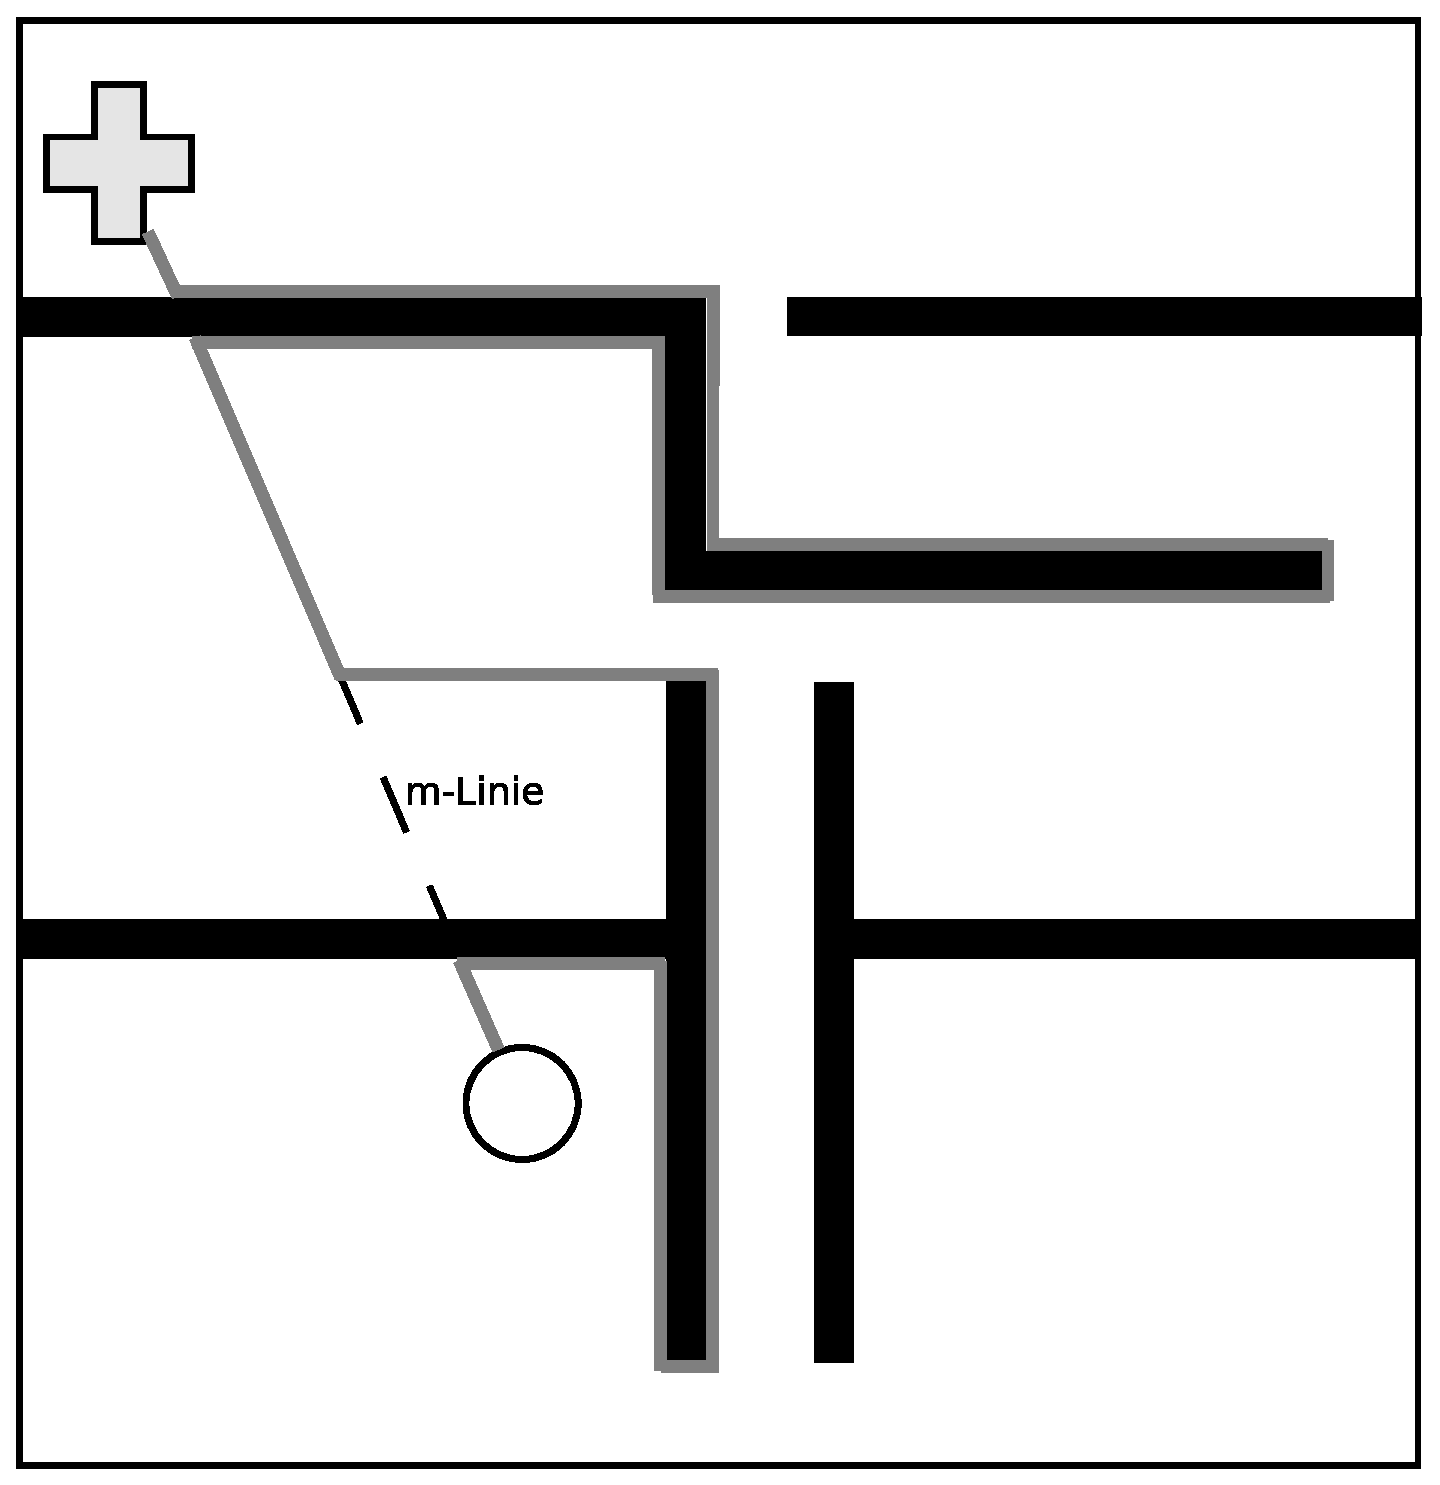
\includegraphics[height=0.35\textwidth]{evaluation/bug_2}
\caption{Veranschaulichung des Bug-2-Algorithmus}
\label{fig:bug_2}
\end{figure}

Abbildung \ref{fig:bug_2} zeigt schematisch einen Grundriss mit einer Person bzw. einem Agenten und einem Notausgang. Die \emph{m-Linie} ist gestrichelt dargestellt, die Wände schwarz.

Nach dem Auslösen der Flucht bewegt sich die Person entlang der m-Linie, bis eine Wand detektiert wird. Eine solche Detektion ist bereits bei dem \emph{random walk} implementiert worden. Es wird von der Person nun ein sogenanntes \emph{wall following} durchgeführt, bis die m-Linie näher am Notausgang passiert wird. Für diesen Schritt kann die initiale m-Linie lokal gespeichert werden oder falls möglich mit der approximierten Position eine neue m-Linie berechnet werden. Die Person bewegt sich erneut entlang der m-Linie.



\floatname{algorithm}{Algorithmus} 
\begin{algorithm}
\caption{Bug-2-Algorithmus}
\label{alg:bug_2}
\begin{algorithmic} 
\STATE last-heading $\leftarrow$ GET-HEADING()
\STATE exit-position $\leftarrow$ GET-NEAREST-EXIT()
\STATE m-line $\leftarrow$ LINE(exit-position, approx-position)
\WHILE{\textit{not rescued}}
\IF{not wall-in-front}
\STATE SET-HEADING(CALCULATE-HEADING(m-line))
\STATE FORWARD 1
\ELSE
\STATE follow-wall $\leftarrow$ true \hfill\emph{; wall detection}
\ENDIF
\WHILE{\textit{follow-wall}}
\IF{on-m-line}
\STATE follow-wall $\leftarrow$ false\hfill\emph{; abort wall following}
\ELSE
\STATE last-heading $\leftarrow$ FOLLOW-WALL(last-heading)\hfill\emph{; wall following}
\ENDIF
\ENDWHILE
\ENDWHILE
\end{algorithmic}
\end{algorithm}



